\documentclass[../tesis.tex]{subfiles}
\begin{document}

% Ruta de imágenes para compilación independiente o desde el main
\graphicspath{{../imagenes/}{imagenes/}}

\chapter{Evaluación de modelos VLM contrastivos multimodales mediante recuperación}

\section{Introducción a los VLM contrastivos}
\label{sec:intro_vlm}

Los Modelos de Visión y Lenguaje (\textit{Vision-Language Models}, VLMs) basados en aprendizaje contrastivo son arquitecturas de redes neuronales diseñadas para proyectar información visual y textual en un espacio latente continuo y compartido. Su objetivo fundamental es evaluar y cuantificar el grado de alineación semántica entre ambas modalidades (imagen y texto).

Estos modelos emplean una arquitectura de doble codificador (\textit{Dual-Encoder}) que procesa cada flujo de datos de manera paralela \citep{myscale_contrastive}:
\begin{itemize}
    \item \textbf{Codificador Visual ($E_v$):} Procesa la información visual (frecuentemente mediante \textit{Vision Transformers} [ViT] o Redes Neuronales Convolucionales avanzadas como ResNet) para transformar la imagen en un vector de características embebidas ($I_k$), denominado \textit{embedding} de imagen.
    \item \textbf{Codificador de Texto ($E_t$):} Procesa la secuencia de tokens del texto (típicamente mediante un \textit{Transformer} codificador o auto-regresivo como BERT o GPT) y convierte el fragmento textual en un \textit{embedding} de texto ($T_k$).
\end{itemize}

Ambos vectores son proyectados mediante matrices de transformación lineal hacia un espacio de dimensión común $D$.

\begin{figure}[htbp]
\centering
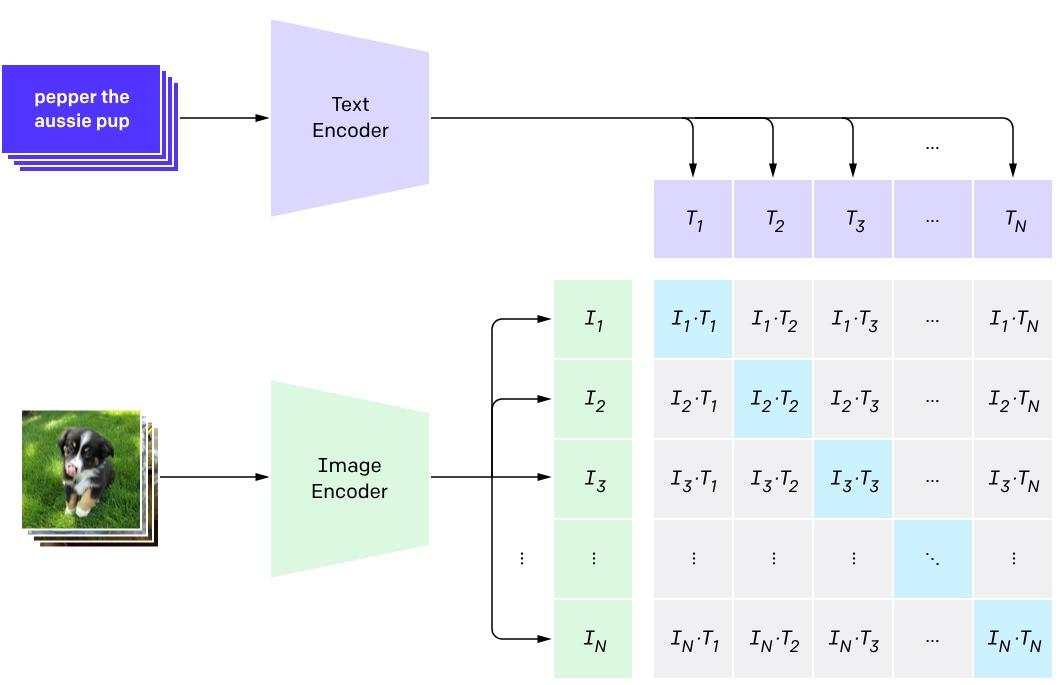
\includegraphics[width=0.8\textwidth]{Tesis/embeddings_vlm.jpeg}
\caption{Diagrama conceptual de la alineación en un espacio latente continuo mediante entrenamiento contrastivo.}
\label{fig:embeddings_vlm}
\end{figure}

El entrenamiento de estas arquitecturas se lleva a cabo utilizando un conjunto de datos formado por pares de imagen y texto $(I_k, T_k)$. Se aplica una función de pérdida InfoNCE simétrica que opera sobre la matriz de similitud del lote (\textit{batch}). Esta función fuerza a que los vectores del par correspondiente ($I_k, T_k$) se aproximen en el espacio latente, mientras aleja la representación visual de cualquier otro texto no correspondiente dentro del mismo lote. La cercanía entre los vectores se evalúa mediante la similitud coseno entre las representaciones normalizadas.

Esta familia de modelos se utiliza ampliamente en tareas de clasificación y recuperación, destacando por su capacidad para operar en esquemas \textit{zero-shot} sin necesidad de ajuste fino (\textit{fine-tuning}) explícito sobre las clases de destino.

\section{Modelo CheXzero}
\label{sec:chexzero}

Una estrategia efectiva para evaluar la capacidad de comprensión multimodal de un modelo de IA en radiología consiste en medir su aptitud para asociar correctamente estudios radiográficos con sus respectivos informes clínicos mediante tareas de recuperación (\textit{retrieval}). En este contexto, un modelo con alta alineación semántica debería identificar el informe clínico original correspondiente a partir de una radiografía dada.

Al revisar el estado del arte de los modelos biomédicos de acceso público, se seleccionó la arquitectura \textbf{CheXzero} \citep{CheXzero_repositorio}, desarrollada por investigadores de las universidades de Stanford y Harvard. El propósito central de CheXzero es la clasificación patológica automatizada en radiografías de tórax (CXR) eliminando la necesidad de anotaciones o etiquetas manuales estructuradas \citep{CheXzero}.

El modelo no fue entrenado desde cero. Se inicializó con los pesos preentrenados oficiales de CLIP (variante ViT-B/32 para la rama visual y un \textit{Transformer} estándar para la rama textual), aprovechando las representaciones lingüísticas y visuales generales aprendidas sobre 400 millones de pares imagen-texto. A partir de esa base, los autores aplicaron aprendizaje contrastivo autosupervisado utilizando el conjunto de datos biomédico MIMIC-CXR desarrollado por el MIT. MIMIC-CXR contiene más de $371\,000$ radiografías de tórax y $227\,000$ informes clínicos anonimizados procedentes del \textit{Beth Israel Deaconess Medical Center} (BIDMC), correspondientes a más de $65\,000$ pacientes \citep{MIMIC-CXR}.

\section{Estrategias de recuperación: estricta, no supervisada y supervisada}
\label{sec:estrategias_retrieval}

La evaluación de la capacidad de recuperación mediante CheXzero en la base de datos local se estructuró bajo tres enfoques con distintos niveles de abstracción semántica:

\begin{enumerate}
    \item \textbf{Recuperación Estricta (Coincidencia Exacta):} Considera un acierto (\textit{hit}) únicamente si el modelo recupera el informe exacto redactado para el paciente analizado. Debido a la presencia de múltiples reportes semánticamente equivalentes en la práctica médica diaria, este enfoque penaliza severamente el desempeño del modelo. Por ello, se incluye como métrica de control para fundamentar la necesidad de agrupamientos semánticos.
    
    \item \textbf{Recuperación No Supervisada (Basada en Clústeres):} Utiliza los \textit{embeddings} de texto de los informes para agruparlos mediante algoritmos de densidad (DBSCAN). Un intento de recuperación se considera exitoso si el modelo selecciona el informe original o cualquier otro informe perteneciente al mismo clúster semántico. Si el informe original fue clasificado como ruido (sin grupo asignado), se exige la coincidencia exacta.
    
    \item \textbf{Recuperación Supervisada (Basada en Mapa de Patologías y Etiquetas):} Asigna a cada reporte un conjunto de etiquetas clínicas (\textit{tags}) normalizadas. La recuperación se considera exitosa si el informe recuperado comparte el mismo conjunto de etiquetas que el informe de origen. Para evaluar coincidencias parciales de forma cuantitativa, se calcula el índice de similitud de Jaccard entre los conjuntos de etiquetas del reporte de origen y el recuperado.
\end{enumerate}

Para implementar el enfoque supervisado, se construyó un mapa de patologías (\textit{pathology map}) estructurado en formato JSON, el cual vincula etiquetas clínicas normalizadas con sus frases descriptivas equivalentes encontradas en los informes (\autoref{tab:mapping_ejemplos}).

\begin{table}[htbp]
\centering
\small
\begin{tabular}{|l|p{8.5cm}|}
\hline
\textbf{Etiqueta Normalizada} & \textbf{Ejemplos de Frases en Informes Curados} \\ \hline
\texttt{normal} & 
• \textit{``No active parenchymal processes are observed''} \newline
• \textit{``S.C.V. compatible with age''} \\ \hline
\texttt{pleural\_adhesions} & 
• \textit{``Peripheral pleural adhesion''} \newline
• \textit{``Left basal pleural adhesions with a sequelae appearance''} \\ \hline
\texttt{hemidiaphragm\_elevation} & 
• \textit{``Elevation of right hemidiaphragm''} \newline
• \textit{``Raised left diaphragm''} \\ \hline
\end{tabular}
\caption{Mapeo entre hallazgos textuales en los informes y etiquetas clínicas normalizadas.}
\label{tab:mapping_ejemplos}
\end{table}


Ante la falta de disponibilidad continua de un especialista radiólogo para la anotación manual de los miles de estudios, se utilizó una herramienta comercial de asistencia basada en modelos de lenguaje (ChatGPT) como apoyo metodológico auxiliar para la extracción, estandarización y normalización inicial de las frases de hallazgos. Posteriormente, las equivalencias propuestas fueron auditadas y consolidadas en el mapa de patologías definitivo.

\paragraph{Limitación metodológica sobre la circularidad del \textit{ground-truth}:} Es fundamental precisar que la generación de la verdad de referencia (\textit{ground-truth}) mediante un LLM introduce un riesgo inherente de circularidad metodológica y sesgos compartidos en las etapas posteriores de evaluación. Al depender las etiquetas diagnósticas de la interpretación algorítmica de los informes históricos —sin una validación directa, independiente y a ciegas realizada por un especialista radiólogo—, la verdad de referencia queda supeditada a la precisión de la extracción textual inicial. En consecuencia, las métricas de rendimiento reportadas en los capítulos posteriores deben interpretarse bajo esta salvedad, dado que eventuales errores de extracción o desalineaciones en las etiquetas de origen podrían propagarse o distorsionar la evaluación comparativa entre modelos.

Al procesar la cohorte de $2\,818$ pacientes del dataset balanceado mediante este mapa de patologías, se identificaron 32 etiquetas clínicas distintas, asignándose un total de $3\,737$ etiquetas. La distribución de las patologías más frecuentes se compone de:
\begin{itemize}
    \item \texttt{aortic\_uncoiling} ($1\,200$ casos)
    \item \texttt{normal} ($971$ casos)
    \item \texttt{aortic\_calcification} ($413$ casos)
    \item \texttt{breast\_implants} ($176$ casos)
    \item \texttt{cardiomegaly} ($160$ casos)
\end{itemize}

Con el fin de ilustrar de forma visual la marcada asimetría y el fenómeno de cola larga (long-tail) en la prevalencia de las patologías del corpus, la \autoref{fig:long_tail} expone la distribución de frecuencias de las etiquetas, complementando el desglose numérico completo presentado en la \autoref{tab:apendice_tags_completos} del Apéndice..

\begin{figure}[htbp]
\centering
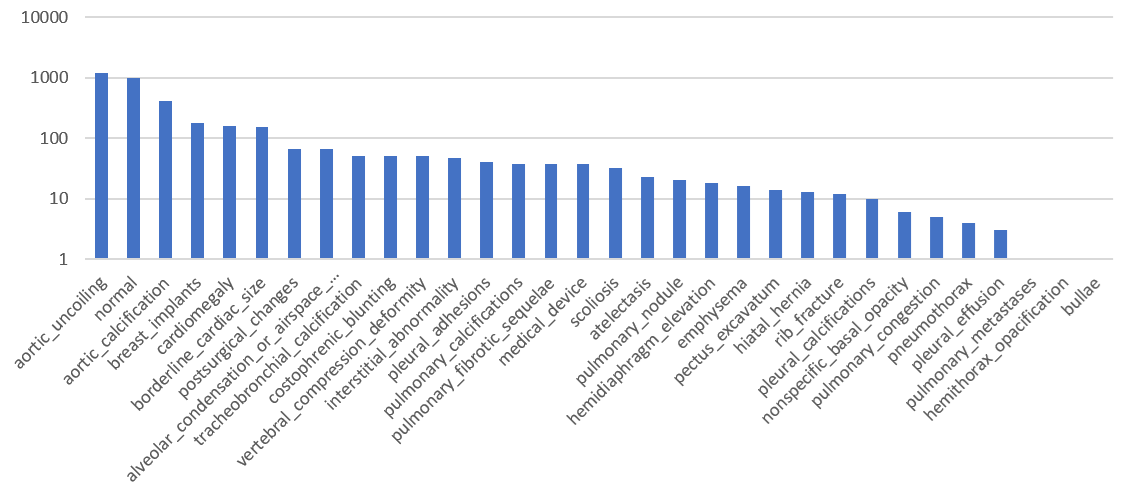
\includegraphics[width=1\textwidth]{Tesis/long_tail.png}
\caption{Distribución de frecuencia en escala logarítmica de los 32 tags clínicos en el corpus de pacientes analizados ($N = 2\,818$),.}
\label{fig:long_tail}
\end{figure}

\section{Pipeline de extracción de embeddings y métricas de desempeño}

El procedimiento computacional se inició cargando la arquitectura base CLIP (ViT-B/32) e inyectando los pesos especializados del punto de control (\textit{checkpoint}) de CheXzero (\autoref{code:chexzero_load}).

Para el procesamiento de imágenes DICOM, los valores de píxel se reescalaron linealmente al rango $[0, 1]$ para mitigar fluctuaciones de luminancia y se convirtieron a formato RGB de 8 bits para garantizar compatibilidad con los canales de entrada de CLIP (\autoref{code:dicom_preprocessing}).

En la fase de extracción de vectores (\textit{embeddings}), en aquellos casos donde el expediente disponía de múltiples proyecciones radiográficas, se aplicó un promediado vectorial (\textit{mean pooling}) de las representaciones visuales. Los informes de texto se tokenizaron truncándolos a un máximo de 77 tokens (límite estructural de CLIP). Finalmente, se aplicó la norma $L_2$ a ambos vectores para proyectarlos sobre una hiperesfera unitaria, permitiendo evaluar la similitud coseno mediante el producto escalar (\autoref{code:embedding_generation}).\\


Para la evaluación supervisada, la similitud de Jaccard entre dos conjuntos de etiquetas $A$ y $B$ se calculó como:
\begin{equation}
    J(A,B) = \frac{|A \cap B|}{|A \cup B|}
\end{equation}

El algoritmo de evaluación contrasta los índices de ordenamiento por similitud coseno generando métricas de precisión Top-1, Top-5 e índice de Jaccard medio (\autoref{code:retrieval_eval}).


\section{Resultados del experimento de recuperación}
\label{sec:resultados_retrieval}

Los resultados globales del proceso de recuperación cruzada (Imagen $\rightarrow$ Texto y Texto $\rightarrow$ Imagen) sobre la cohorte inicial de $2\,818$ pacientes se resumen en la \autoref{tab:retrieval_resultados_globales}.

\begin{table}[htbp]
\centering
\small
\makebox[\textwidth][c]{
\begin{tabular}{llcc}
\toprule
\textbf{Enfoque de Evaluación} & \textbf{Métrica} & \textbf{Imagen $\rightarrow$ Texto (\%)} & \textbf{Texto $\rightarrow$ Imagen (\%)} \\
\midrule
\textbf{Retrieval Estricto} & Top-1 Accuracy & 0.4 & 0.5 \\
\textit{(Paciente exacto)} & Top-5 Accuracy & 1.5 & 1.4 \\
\midrule
\textbf{No Supervisado} & Top-1 (Mismo Clúster) & 1.1 & 31.2 \\
\textit{(Clustering DBSCAN)} & Top-5 (Mismo Clúster) & 5.4 & 38.5 \\
\midrule
\textbf{Supervisado} & Mean Jaccard@1 & 16.8 & 39.9 \\
\textit{(Pathology Map / Tags)} & Mean Best Jaccard@5 & 40.6 & 74.7 \\
\bottomrule
\end{tabular}
}
\caption{Desempeño del sistema de recuperación multimodal con CheXzero sobre la base de $2\,818$ pacientes.}
\label{tab:retrieval_resultados_globales}
\end{table}

Los resultados demuestran un rendimiento sumamente bajo en la recuperación estricta de texto a partir de la imagen ($0.43\%$ en Top-1), lo que confirma la hipótesis de que diferentes informes con redacciones distintas describen hallazgos clínicos equivalentes. No obstante, al analizar las métricas supervisadas y no supervisadas, se observó que la presencia masiva de etiquetas de rutina (\texttt{normal} y \texttt{aortic\_uncoiling}) distorsionaba las evaluaciones de similitud. La alteración \texttt{aortic\_uncoiling} (aorta desenrollada) constituye un hallazgo senil benigno frecuentemente asociado a estudios normales.

Para corregir esta distorsión, se aplicó una segunda fase de filtrado: se fijó un límite superior de 500 pacientes para la etiqueta \texttt{normal} y se eliminaron los registros cuya única anotación fuera \texttt{aortic\_uncoiling}. Esto redujo el dataset de $2\,818$ a $1\,749$ expedientes ($500$ normales y $602$ con elongación aórtica). La reevaluación sobre esta cohorte purgada produjo las métricas presentadas en la \autoref{tab:retrieval_resultados_filtrados}.

\begin{table}[htbp]
\centering
\small
\makebox[\textwidth][c]{
\begin{tabular}{llcc}
\toprule
\textbf{Enfoque de Evaluación} & \textbf{Métrica} & \textbf{Imagen $\rightarrow$ Texto (\%)} & \textbf{Texto $\rightarrow$ Imagen (\%)} \\
\midrule
\textbf{Retrieval Estricto} & Top-1 Accuracy & 0.7 & 0.9 \\
\textit{(Paciente exacto)} & Top-5 Accuracy & 2.3 & 2.7 \\
\midrule
\textbf{No Supervisado} & Top-1 (Mismo Clúster) & 1.1 & 14.6 \\
\textit{(Clustering DBSCAN)} & Top-5 (Mismo Clúster) & 4.8 & 37.1 \\
\midrule
\textbf{Supervisado} & Mean Jaccard@1 & 14.5 & 27.5 \\
\textit{(Pathology Map / Tags)} & Mean Best Jaccard@5 & 39.6 & 65.2 \\
\bottomrule
\end{tabular}
}
\caption{Desempeño del sistema de recuperación tras la eliminación de etiquetas benignas sobrepresentadas ($1\,749$ pacientes).}
\label{tab:retrieval_resultados_filtrados}
\end{table}

A pesar del filtrado, persistió un fuerte desbalance de cola larga (\textit{long-tail distribution}): de las 32 patologías, 26 registraban menos de 100 ocurrencias y 7 aparecían en menos de 10 casos.

Como experimento final, se implementó una estrategia de muestreo llamada \textbf{Selección Codiciosa por Minorías} (\textit{Greedy Minority-First Selection}). Esta técnica descartó patologías con menos de 30 apariciones globales y ordenó a los pacientes priorizando las etiquetas más infrecuentes, estableciendo un cupo máximo estricto de 50 pacientes por clase (\autoref{code:balanceo_greedy}). La evaluación sobre este subconjunto balanceado por patologías infrecuentes produjo los resultados expuestos en la \autoref{tab:retrieval_resultados_balanceados}.

\begin{table}[htbp]
\centering
\small
\makebox[\textwidth][c]{
\begin{tabular}{llcc}
\toprule
\textbf{Enfoque de Evaluación} & \textbf{Métrica} & \textbf{Imagen $\rightarrow$ Texto (\%)} & \textbf{Texto $\rightarrow$ Imagen (\%)} \\
\midrule
\textbf{Retrieval Estricto} & Top-1 Accuracy & 2.9 & 3.4 \\
\textit{(Paciente exacto)} & Top-5 Accuracy & 8.6 & 11.4 \\
\midrule
\textbf{No Supervisado} & Top-1 (Mismo Clúster) & 3.4 & 8.3 \\
\textit{(Clustering DBSCAN)} & Top-5 (Mismo Clúster) & 10.7 & 20.3 \\
\midrule
\textbf{Supervisado} & Mean Jaccard@1 & 16.1 & 26.1 \\
\textit{(Pathology Map / Tags)} & Mean Best Jaccard@5 & 40.2 & 50.7 \\
\bottomrule
\end{tabular}
}
\caption{Desempeño de recuperación tras aplicar la estrategia de balanceo por Selección Codiciosa por Minorías.}
\label{tab:retrieval_resultados_balanceados}
\end{table}

\section{Discusión y conclusiones del capítulo}
\label{sec:discusion_ch2}

El análisis experimental evidencia que la tarea de recuperación cruzada libre (\textit{free-form cross-modal retrieval}) mediante modelos VLM contrastivos sin adaptar está condicionada por la naturaleza multietiqueta de las radiografías y la variabilidad léxica de los informes. Aunque CheXzero ha demostrado métricas sobresalientes en la literatura internacional \citep{CheXzero, Tiu_et_al._2022}, su rendimiento en tareas de recuperación abierta sobre un conjunto de datos local es limitado (alcanzando un índice de Jaccard medio del $16\%$ al $40\%$ en Top-1 y Top-5).

Esta discrepancia sugiere que la evaluación adecuada para medir el conocimiento clínico en un VLM contrastivo no debe basarse en la recuperación de texto libre entre pacientes heterogéneos, sino en esquemas de \textbf{Clasificación Zero-Shot}. En dichos esquemas, las patologías se evalúan utilizando plantillas fijas de texto (\textit{prompts} como \textit{``A frontal chest radiograph demonstrating [patología]''}) y calculando el Área Bajo la Curva ROC (AUROC) o el Coeficiente de Correlación de Matthews (MCC).

Asimismo, estos hallazgos justifican la necesidad metodológica abordada en los siguientes capítulos de esta tesis: para lograr la generación automática de informes precisos en entornos locales, no basta con emplear representaciones contrastivas congeladas de un VLM preentrenado; se requiere el desarrollo de modelos generativos específicos adaptados al dominio clínico mediante arquitecturas dedicadas y estrategias de ajuste fine-tuning o aprendizaje autosupervisado.

\end{document}